\documentclass[../main.tex]{subfiles}



\begin{document}

\chapter{}
\label{cha:cha_11}


\section{}
\begin{enumerate}[label=\bfseries(\alph*)]
\item The first iteration can be implemented as
\bigbreak$
\begin{aligned}
&x_{1}=\dfrac{41+0.4 x_{2}}{0.8}=\dfrac{41+0.4(0)}{0.8}=51.25 \\\\
&x_{2}=\dfrac{25+0.4 x_{1}+0.4 x_{3}}{0.8}=\dfrac{25+0.4(51.25)+0.4(0)}{0.8}=56.875 \\\\
&x_{3}=\dfrac{105+0.4 x_{2}}{0.8}=\dfrac{105+0.4(56.875)}{0.8}=159.6875
\end{aligned}$
\bigbreak
Second iteration:
\bigbreak$
\begin{aligned}
&x_{1}=\dfrac{41+0.4(56.875)}{0.8}=79.6875 \\\\
&x_{2}=\dfrac{25+0.4(79.6875)+0.4(159.6875)}{0.8}=150.9375 \\\\
&x_{3}=\dfrac{105+0.4(150.9375)}{0.8}=206.7188
\end{aligned}$
\bigbreak
The error estimates can be computed as
\bigbreak$
\begin{aligned}
&\varepsilon_{a, 1}=\left|\dfrac{79.6875-51.25}{79.6875}\right| \times 100 \%=35.69 \% \\\\
&\varepsilon_{a, 2}=\left|\dfrac{150.9375-56.875}{150.9375}\right| \times 100 \%=62.32 \% \\\\
&\varepsilon_{a, 3}=\left|\dfrac{206.7188-159.6875}{206.7188}\right| \times 100 \%=22.75 \%
\end{aligned}$
\bigbreak
The remainder of the calculation proceeds until all the errors fall below the stopping criterion of $5 \%$. \smallbreak The entire computation can be summarized as
\bigbreak
\begin{tabular}{ccrrr}
\Xhline{1.5pt}
iteration & unknown & \multicolumn{1}{c}{value} & \multicolumn{1}{c}{$\varepsilon_{a}$} & maximum $\varepsilon_{a}$ \\
\hline
1 & $x_{1}$ & $51.25$ & $100.00 \%$ &  \\
 & $x_{2}$ & $56.875$ & $100.00 \%$ &  \\
 & $x_{3}$ & $159.6875$ & $100.00 \%$ & $100.00 \%$ \\
\hline
2 & $x_{1}$ & $79.6875$ & $35.69 \%$ &  \\
 & $x_{2}$ & $150.9375$ & $62.32 \%$ &  \\
 & $x_{3}$ & $206.7188$ & $22.75 \%$ & $62.32 \%$ \\
\hline
3 & $x_{1}$ & $126.7188$ & $37.11 \%$ &  \\
 & $x_{2}$ & $197.9688$ & $23.76 \%$ &  \\
 & $x_{3}$ & $230.2344$ & $10.21 \%$ & $37.11 \%$ \\
\hline
4 & $x_{1}$ & $150.2344$ & $15.65 \%$ &  \\
 & $x_{2}$ & $221.4844$ & $10.62 \%$ &  \\
 & $x_{3}$ & $241.9922$ & $4.86 \%$ & $15.65 \%$ \\
\hline
5 & $x_{1}$ & $161.9922$ & $7.26 \%$ &  \\
 & $x_{2}$ & $233.2422$ & $5.04 \%$ &  \\
 & $x_{3}$ & $247.8711$ & $2.37 \%$ & $7.26 \%$ \\
\hline
6 & $x_{1}$ & $167.8711$ & $3.50 \%$ &  \\
 & $x_{2}$ & $239.1211$ & $2.46 \%$ &  \\
 & $x_{3}$ & $250.8105$ & $1.17 \%$ & $3.50 \%$ \\
\Xhline{1.5pt}
\end{tabular}
\bigbreak
Thus, after 6 iterations, the maximum error is $3.5 \%$ and we arrive at the result: $x_{1}=$\smallbreak $167.8711, x_{2}=239.1211$ and $x_{3}=250.8105$.
\bigbreak
\item The same computation can be developed with relaxation where $\lambda=1.2$.
\bigbreak
$\underline{\text { First iteration: }}$
\bigbreak
$x_{1}=\dfrac{41+0.4 x_{2}}{0.8}=\dfrac{41+0.4(0)}{0.8}=51.25$
\bigbreak
Relaxation yields: $x_{1}=1.2(51.25)-0.2(0)=61.5$
\bigbreak
$x_{2}=\dfrac{25+0.4 x_{1}+0.4 x_{3}}{0.8}=\dfrac{25+0.4(61.5)+0.4(0)}{0.8}=62$
\bigbreak
Relaxation yields: $x_{2}=1.2(62)-0.2(0)=74.4$
\bigbreak
$x_{3}=\dfrac{105+0.4 x_{2}}{0.8}=\dfrac{105+0.4(62)}{0.8}=168.45$
\bigbreak
Relaxation yields: $x_{3}=1.2(168.45)-0.2(0)=202.14$
\bigbreak
$\underline{\text { Second iteration: }}$
\bigbreak
$x_{1}=\dfrac{41+0.4(62)}{0.8}=88.45$
\bigbreak
Relaxation yields: $x_{1}=1.2(88.45)-0.2(61.5)=93.84$
\bigbreak
$x_{2}=\dfrac{25+0.4(93.84)+0.4(202.14)}{0.8}=179.24$
\bigbreak
Relaxation yields: $x_{2}=1.2(179.24)-0.2(74.4)=200.208$
\bigbreak
$x_{3}=\dfrac{105+0.4(200.208)}{0.8}=231.354$
\bigbreak
Relaxation yields: $x_{3}=1.2(231.354)-0.2(202.14)=237.1968$
\bigbreak
The error estimates can be computed as
\bigbreak$
\begin{aligned}
&\varepsilon_{a, 1}=\left|\dfrac{93.84-61.5}{93.84}\right| \times 100 \%=34.46 \% \\\\
&\varepsilon_{a, 2}=\left|\dfrac{200.208-74.4}{200.208}\right| \times 100 \%=62.84 \% \\\\
&\varepsilon_{a, 3}=\left|\dfrac{237.1968-202.14}{237.1968}\right| \times 100 \%=14.78 \%
\end{aligned}$
\bigbreak
The remainder of the calculation proceeds until all the errors fall below the stopping criterion of $5 \%$. \smallbreak The entire computation can be summarized as
\bigbreak
\begin{tabular}{ccrrcr}
\Xhline{1.5pt}
iteration & unknown & \multicolumn{1}{c}{value} & relaxation & $\varepsilon_{\mathrm{a}}$ & maximum $\varepsilon_{\mathrm{a}}$ \\
\hline
1 & $x_{1}$ & $51.25$ & $61.5$ & $100.00 \%$ &  \\
 & $x_{2}$ & 62 & $74.4$ & $100.00 \%$ &  \\
 & $x_{3}$ & $168.45$ & $202.14$ & $100.00 \%$ & $100.000 \%$ \\
\hline
2 & $x_{1}$ & $88.45$ & $93.84$ & $34.46 \%$ &  \\
 & $x_{2}$ & $179.24$ & $200.208$ & $62.84 \%$ &  \\
 & $x_{3}$ & $231.354$ & $237.1968$ & $14.78 \%$ & $62.839 \%$ \\
\hline
3 & $x_{1}$ & $151.354$ & $162.8568$ & $42.38 \%$ &  \\
 & $x_{2}$ & $231.2768$ & $237.49056$ & $15.70 \%$ &  \\
 & $X_{3}$ & $249.99528$ & $252.55498$ & $6.08 \%$ & $42.379 \%$ \\
\hline
4 & $x_{1}$ & $169.99528$ & $171.42298$ & $5.00 \%$ &  \\
 & $x_{2}$ & $243.23898$ & $244.38866$ & $2.82 \%$ &  \\
 & $X_{3}$ & $253.44433$ & $253.6222$ & $0.42 \%$ & $4.997 \%$ \\
\Xhline{1.5pt}
\end{tabular}
\bigbreak
Thus, relaxation speeds up convergence. After 6 iterations, the maximum error is $4.997 \%$ and we arrive at the result: $x_{1}=171.423, x_{2}=244.389$ and $x_{3}=253.622$.
\bigbreak


\section{}

The first iteration can be implemented as
\bigbreak$
\begin{aligned}
&x_{1}=\dfrac{27-2 x_{2}+x_{3}}{10}=\dfrac{27-2(0)+0}{10}=2.7 \\\\
&x_{2}=\dfrac{-61.5+3 x_{1}-2 x_{3}}{-6}=\dfrac{-61.5+3(2.7)-2(0)}{-6}=8.9 \\\\
&x_{3}=\dfrac{-21.5-x_{1}-x_{2}}{5}=\dfrac{-21.5-(2.7)-8.9}{5}=-6.62
\end{aligned}$
\bigbreak
Second iteration:
\bigbreak$
\begin{aligned}
&x_{1}=\dfrac{27-2(8.9)-6.62}{10}=0.258 \\\\
&x_{2}=\dfrac{-61.5+3(0.258)-2(-6.62)}{-6}=7.914333 \\\\
&x_{3}=\dfrac{-21.5-(0.258)-7.914333}{5}=-5.934467
\end{aligned}$
\bigbreak
The error estimates can be computed as
\bigbreak$
\begin{aligned}
&\varepsilon_{a, 1}=\left|\dfrac{0.258-2.7}{0.258}\right| \times 100 \%=947 \% \\\\
&\varepsilon_{a, 2}=\left|\dfrac{7.914333-8.9}{7.914333}\right| \times 100 \%=12.45 \% \\\\
&\varepsilon_{a, 3}=\left|\dfrac{-5.934467-(-6.62)}{-5.934467}\right| \times 100 \%=11.55 \%
\end{aligned}$
\bigbreak
The remainder of the calculation proceeds until all the errors fall below the stopping\smallbreak criterion of $5 \%$. The entire computation can be summarized as
\bigbreak
$\begin{array}{ccrrr}
\Xhline{1.5pt} \text { iteration } & \text { unknown } & \multicolumn{1}{c}{\text { value }} & \multicolumn{1}{c}{\varepsilon_{a}} & \text { maximum } \varepsilon_{a} \\
\hline 1 & x_{1} & 2.7 & 100.00 \% & \\
& x_{2} & 8.9 & 100.00 \% & \\
& x_{3} & -6.62 & 100.00 \% & 100 \% \\
\hline 2 & x_{1} & 0.258 & 946.51 \% & \\
& x_{2} & 7.914333 & 12.45 \% & \\
& x_{3} & -5.93447 & 11.55 \% & 946 \% \\
\hline 3 & x_{1} & 0.523687 & 50.73 \% & \\
& x_{2} & 8.010001 & 1.19 \% & \\
& x_{3} & -6.00674 & 1.20 \% & 50.73 \% \\
\hline 4 & x_{1} & 0.497326 & 5.30 \% & \\
& x_{2} & 7.999091 & 0.14 \% & \\
& x_{3} & -5.99928 & 0.12 \% & 5.30 \% \\
\hline 5 & x_{1} & 0.500253 & 0.59 \% & \\
& x_{2} & 8.000112 & 0.01 \% & \\
& x_{3} & -6.00007 & 0.01 \% & 0.59 \% \\
\Xhline{1.5pt}
\end{array}$
\bigbreak
Thus, after 5 iterations, the maximum error is $0.59 \%$ and we arrive at the result: $x_{1}=$\smallbreak $0.500253, x_{2}=8.000112$ and $x_{3}=-6.00007$.
\bigbreak


\section{}

The first iteration can be implemented as
\bigbreak$
\begin{aligned}
&x_{1}=\dfrac{27-2 x_{2}+x_{3}}{10}=\dfrac{27-2(0)+0}{10}=2.7\\\\
&x_{2}=\dfrac{-61.5+3 x_{1}-2 x_{3}}{-6}=\dfrac{-61.5+3(0)-2(0)}{-6}=10.25 \\\\
&x_{3}=\dfrac{-21.5-x_{1}-x_{2}}{5}=\dfrac{-21.5-0-0}{5}=-4.3
\end{aligned}$
\bigbreak
Second iteration:
\bigbreak$
\begin{aligned}
&x_{1}=\dfrac{27-2(10.25)-4.3}{10}=0.22 \\\\
&x_{2}=\dfrac{-61.5+3(2.7)-2(-4.3)}{-6}=7.466667 \\\\
&x_{3}=\dfrac{-21.5-(2.7)-10.25}{5}=-6.89
\end{aligned}$
\bigbreak
The error estimates can be computed as
\bigbreak$
\begin{aligned}
&\varepsilon_{a, 1}=\left|\dfrac{0.22-2.7}{0.258}\right| \times 100 \%=1127 \% \\\\
&\varepsilon_{a, 2}=\left|\dfrac{7.466667-10.25}{7.466667}\right| \times 100 \%=37.28 \% \\\\
&\varepsilon_{a, 3}=\left|\dfrac{-6.89-(-4.3)}{-6.89}\right| \times 100 \%=37.59 \%
\end{aligned}$
\bigbreak
The remainder of the calculation proceeds until all the errors fall below the stopping\smallbreak criterion of $5 \%$. The entire computation can be summarized as
\bigbreak

$\begin{array}{ccrrr}
\Xhline{1.5pt} \text { iteration } & \text { unknown } & \multicolumn{1}{c}{\text { value }} & \multicolumn{1}{c}{\varepsilon_{a}} & \text { maximum } \varepsilon_{a} \\
\hline 1 & x_{1} & 2.7 & 100.00 \% & \\
& x_{2} & 10.25 & 100.00 \% & \\
& x_{3} & -4.3 & 100.00 \% & 100.00 \% \\
\hline 2 & x_{1} & 0.22 & 1127.27 \% & \\
& x_{2} & 7.466667 & 37.28 \% & \\
& x_{3} & -6.89 & 37.59 \% & 1127.27 \% \\
\hline 3 & x_{1} & 0.517667 & 57.50 \% & \\
& x_{2} & 7.843333 & 4.80 \% & \\
& x_{3} & -5.83733 & 18.03 \% & 57.50 \% \\
\hline 4 & x_{1} & 0.5476 & 5.47 \% & \\
& x_{2} & 8.045389 & 2.51 \% & \\
& x_{3} & -5.9722 & 2.26 \% & 5.47 \% \\
\hline 5 & x_{1} & 0.493702 & 10.92 \% & \\
& x_{2} & 7.985467 & 0.75 \% & \\
& x_{3} & -6.0186 & 0.77 \% & 10.92 \% \\
\hline 6 & x_{1} & 0.501047 & 1.47 \% & \\
& x_{2} & 7.99695 & 0.14 \% & \\
& x_{3} & -5.99583 & 0.38 \% & 1.47 \% \\
\Xhline{1.5pt}
\end{array}$
\bigbreak
Thus, after 6 iterations, the maximum error is $1.47 \%$ and we arrive at the result: $x_{1}=$\smallbreak $0.501047, x_{2}=7.99695$ and $x_{3}=-5.99583$.
\bigbreak


\section{}

The first iteration can be implemented as
\bigbreak$
\begin{aligned}
&c_{1}=\dfrac{3800+3 c_{2}+c_{3}}{15}=\dfrac{3800+3(0)+0}{15}=253.3333 \\\\
&c_{2}=\dfrac{1200+3 c_{1}+6 c_{3}}{18}=\dfrac{1200+3(253.3333)+6(0)}{18}=108.8889 \\\\
&c_{3}=\dfrac{2350+4 c_{1}+c_{2}}{12}=\dfrac{2350+4(253.3333)+108.8889}{12}=289.3519
\end{aligned}$
\bigbreak
Second iteration:
\bigbreak$
\begin{aligned}
&c_{1}=\dfrac{3800+3(108.889)+289.3519}{15}=294.4012 \\\\
&c_{2}=\dfrac{1200+3(294.4012)+6(289.3519)}{18}=212.1842 \\\\
&c_{3}=\dfrac{2350+4(294.4012)+212.1842}{12}=311.6491
\end{aligned}$
\bigbreak
The error estimates can be computed as
\bigbreak$
\begin{aligned}
&\varepsilon_{a, 1}=\left|\dfrac{294.4012-253.3333}{294.4012}\right| \times 100 \%=13.95 \% \\\\
&\varepsilon_{a, 2}=\left|\dfrac{212.1842-108.8889}{212.1842}\right| \times 100 \%=48.68 \% \\\\
&\varepsilon_{a, 3}=\left|\dfrac{311.6491-289.3519}{311.6491}\right| \times 100 \%=7.15 \%
\end{aligned}$
\bigbreak
The remainder of the calculation can be summarized as
\bigbreak

$\begin{array}{ccccr}
\Xhline{1.5pt} \text { iteration } & \text { unknown } & \text { value } & \varepsilon_{a} & \text { maximum } \varepsilon_{a} \\
\hline 1 & x_{1} & 253.3333 & 100.00 \% & \\
& x_{2} & 108.8889 & 100.00 \% & \\
& x_{3} & 289.3519 & 100.00 \% & 100.00 \% \\
\hline 2 & x_{1} & 294.4012 & 13.95 \% & \\
& x_{2} & 212.1842 & 48.68 \% & \\
& x_{3} & 311.6491 & 7.15 \% & 48.68 \% \\
\hline 3 & x_{1} & 316.5468 & 7.00 \% & \\
& x_{2} & 223.3075 & 4.98 \% & \\
& x_{3} & 319.9579 & 2.60 \% & 7.00 \% \\
\hline 4 & x_{1} & 319.3254 & 0.87 \% & \\
& x_{2} & 226.5402 & 1.43 \% & \\
& x_{3} & 321.1535 & 0.37 \% & 1.43 \% \\
\hline 5 & x_{1} & 320.0516 & 0.23 \% & \\
& x_{2} & 227.0598 & 0.23 \% & \\
& x_{3} & 321.4388 & 0.09 \% & 0.23 \% \\
\Xhline{1.5pt}
\end{array}$

\bigbreak
Note that after several more iterations, we arrive at the result: $x_{1}=320.2073, x_{2}=227.2021$ and $x_{3}=321.5026$.
\bigbreak
\end{enumerate}


\section{}

The equations must first be rearranged so that they are diagonally dominant
\bigbreak$
\begin{aligned}
&-8 x_{1}+x_{2}-2 x_{3}=-20 \\
&2 x_{1}-6 x_{2}-x_{3}=-38 \\
&-3 x_{1}-x_{2}+7 x_{3}=-34
\end{aligned}$
\bigbreak
\begin{enumerate}[label=\bfseries(\alph*)]
\item The first iteration can be implemented as
\bigbreak$
\begin{aligned}
&x_{1}=\dfrac{-20-x_{2}+2 x_{3}}{-8}=\dfrac{-20-0+2(0)}{-8}=2.5 \\\\
&x_{2}=\dfrac{-38-2 x_{1}+x_{3}}{-6}=\dfrac{-38-2(2.5)+0}{-6}=7.166667 \\\\
&x_{3}=\dfrac{-34+3 x_{1}+x_{2}}{7}=\dfrac{-34+3(2.5)+7.166667}{7}=-2.761905
\end{aligned}$
\bigbreak
Second iteration:
\bigbreak$
\begin{aligned}
&x_{1}=\dfrac{-20-7.166667+2(-2.761905)}{-8}=4.08631 \\\\
&x_{2}=\dfrac{-38-2 x_{1}+x_{3}}{-6}=\dfrac{-38-2(4.08631)+(-2.761905)}{-6}=8.155754 \\\\
&x_{3}=\dfrac{-34+3 x_{1}+x_{2}}{7}=\dfrac{-34+3(4.08631)+8.155754}{7}=-1.94076
\end{aligned}$
\bigbreak
The error estimates can be computed as
\bigbreak$
\begin{aligned}
&\varepsilon_{a, 1}=\left|\dfrac{4.08631-2.5}{4.08631}\right| \times 100 \%=38.82 \% \\\\
&\varepsilon_{a, 2}=\left|\dfrac{8.155754-7.166667}{8.155754}\right| \times 100 \%=12.13 \% \\\\
&\varepsilon_{a, 3}=\left|\dfrac{-1.94076-(-2.761905)}{-1.94076}\right| \times 100 \%=42.31 \%
\end{aligned}$
\bigbreak
The remainder of the calculation proceeds until all the errors fall below the stopping\smallbreak criterion of $5 \%$. The entire computation can be summarized as
\bigbreak
$\begin{array}{ccrcr}
\Xhline{1.5pt} \text { iteration } & \text { unknown } & \multicolumn{1}{c}{\text { value }} & \varepsilon_{a} & \text { maximum } \varepsilon_{a} \\
\hline 0 & x_{1} & 0 & & \\
& x_{2} & 0 & & \\
& x_{3} & 0 & & \\
\hline 1 & x_{1} & 2.5 & 100.00 \% & \\
& x_{2} & 7.166667 & 100.00 \% & \\
& x_{3} & -2.7619 & 100.00 \% & 100.00 \% \\
\hline 2 & x_{1} & 4.08631 & 38.82 \% & \\
& x_{2} & 8.155754 & 12.13 \% & \\
& x_{3} & -1.94076 & 42.31 \% & 42.31 \% \\
\hline 3 & x_{1} & 4.004659 & 2.04 \% & \\
& x_{2} & 7.99168 & 2.05 \% & \\
& x_{3} & -1.99919 & 2.92 \% & 2.92 \% \\
\Xhline{1.5pt}
\end{array}$
\bigbreak
Thus, after 3 iterations, the maximum error is $2.92 \%$ and we arrive at the result: $x_{1}=$\smallbreak $4.004659, x_{2}=7.99168$ and $x_{3}=-1.99919$.
\bigbreak
\item The same computation can be developed with relaxation where $\lambda=1.2$.
\bigbreak
\underline{First iteration:}
\bigbreak

$x_{1}=\dfrac{-20-x_{2}+2 x_{3}}{-8}=\dfrac{-20-0+2(0)}{-8}=2.5$
\bigbreak
Relaxation yields: $x_{1}=1.2(2.5)-0.2(0)=3$
\bigbreak
$x_{2}=\dfrac{-38-2 x_{1}+x_{3}}{-6}=\dfrac{-38-2(3)+0}{-6}=7.333333$
\bigbreak
Relaxation yields: $x_{2}=1.2(7.333333)-0.2(0)=8.8$
\bigbreak
$x_{3}=\dfrac{-34+3 x_{1}+x_{2}}{7}=\dfrac{-34+3(3)+8.8}{7}=-2.3142857$
\bigbreak
Relaxation yields: $x_{3}=1.2(-2.3142857)-0.2(0)=-2.7771429$ 
\bigbreak
\underline{ Second iteration:}
\bigbreak
$x_{1}=\dfrac{-20-x_{2}+2 x_{3}}{-8}=\dfrac{-20-8.8+2(-2.7771429)}{-8}=4.2942857$
\bigbreak
Relaxation yields: $x_{1}=1.2(4.2942857)-0.2(3)=4.5531429$
\bigbreak
$x_{2}=\dfrac{-38-2 x_{1}+x_{3}}{-6}=\dfrac{-38-2(4.5531429)-2.7771429}{-6}=8.3139048$
\bigbreak
Relaxation yields: $x_{2}=1.2(8.3139048)-0.2(8.8)=8.2166857$
\bigbreak
$x_{3}=\dfrac{-34+3 x_{1}+x_{2}}{7}=\dfrac{-34+3(4.5531429)+8.2166857}{7}=-1.7319837$
\bigbreak
Relaxation yields: $x_{3}=1.2(-1.7319837)-0.2(-2.7771429)=-1.5229518$
\bigbreak
The error estimates can be computed as
\bigbreak$
\begin{aligned}
&\varepsilon_{a, 1}=\left|\dfrac{4.5531429-3}{4.5531429}\right| \times 100 \%=34.11 \% \\\\
&\varepsilon_{a, 2}=\left|\dfrac{8.2166857-8.8}{8.2166857}\right| \times 100 \%=7.1 \% \\\\
&\varepsilon_{a, 3}=\left|\dfrac{-1.5229518-(-2.7771429)}{-1.5229518}\right| \times 100 \%=82.35 \%
\end{aligned}$
\bigbreak
The remainder of the calculation proceeds until all the errors fall below the stopping\smallbreak criterion of $5 \%$. The entire computation can be summarized as
\bigbreak

\begin{tabular}{crrrrr}
\Xhline{1.5pt}
iteration & unknown & value & relaxation &\multicolumn{1}{c}{$\varepsilon_{a}$} & maximum $\varepsilon_{a}$ \\
\hline
1 & $x_{1}$ & $2.5$ & 3 & $100.00 \%$ &  \\
 & $x_{2}$ & $7.3333333$ & $8.8$ & $100.00 \%$ &  \\
 & $x_{3}$ & $-2.314286$ & $-2.777143$ & $100.00 \%$ & $100.000 \%$ \\
\hline
2 & $x_{1}$ & $4.2942857$ & $4.5531429$ & $34.11 \%$ &  \\
 & $x_{2}$ & $8.3139048$ & $8.2166857$ & $7.10 \%$ &  \\
 & $x_{3}$ & $-1.731984$ & $-1.522952$ & $82.35 \%$ & $82.353 \%$ \\
\hline
3 & $x_{1}$ & $3.9078237$ & $3.7787598$ & $20.49 \%$ &  \\
 & $x_{2}$ & $7.8467453$ & $7.7727572$ & $5.71 \%$ &  \\
 & $x_{3}$ & $-2.12728$ & $-2.248146$ & $32.26 \%$ & $32.257 \%$ \\
\hline
4 & $x_{1}$ & $4.0336312$ & $4.0846055$ & $7.49 \%$ &  \\
 & $x_{2}$ & $8.0695595$ & $8.12892$ & $4.38 \%$ &  \\
 & $x_{3}$ & $-1.945323$ & $-1.884759$ & $19.28 \%$ & $19.280 \%$ \\
\hline
5 & $x_{1}$ & $3.9873047$ & $3.9678445$ & $2.94 \%$ &  \\
 & $x_{2}$ & $7.9700747$ & $7.9383056$ & $2.40 \%$ &  \\
 & $x_{3}$ & $-2.022594$ & $-2.050162$ & $8.07 \%$ & $8.068 \%$ \\
\hline
6 & $x_{1}$ & $4.0048286$ & $4.0122254$ & $1.11 \%$ &  \\
 & $x_{2}$ & $8.0124354$ & $8.0272613$ & $1.11 \%$ &  \\
 & $x_{3}$ & $-1.990866$ & $-1.979007$ & $3.60 \%$ & $3.595 \%$ \\
\Xhline{1.5pt}
\end{tabular}
\bigbreak
Thus, relaxation actually seems to retard convergence. After 6 iterations, the maximum error is $3.595 \%$ and we arrive at the result: $x_{1}=4.0122254, x_{2}=8.0272613$ and $x_{3}=$ $-1.979007 .$
\bigbreak


\section{}
As ordered, none of the sets will converge. However, if Set 1 and 3 are reordered so that they are diagonally dominant, they will converge on the solution of $(1,1,1)$.
\bigbreak


Set 1: \quad\hspace*{0.1cm}$8 x+3 y+z=12$

\quad\hspace*{1cm}$2 x+4 y-z=5$

\quad\hspace*{0.85cm}$-6 x\quad    +7 z=1$

\bigbreak
Set 3: \quad$3 x+y-z=3$

\quad\hspace*{0.9cm}$x+4 y-z=4$

\quad\hspace*{0.9cm}$x+y+5 z=7$
\bigbreak

Because it is not diagonally dominant, Set 2 will not converge on the correct solution of (1, $1,1)$. However, it will also not diverge. Rather, it will oscillate. The way that this occurs depends on how the equations are ordered. For example, if they can be ordered as
\bigbreak$
\begin{gathered}
-2 x+4 y-5 z=-3 \\
\quad\quad2 y-z   	=1 \\
-x+3 y+5 z=7
\end{gathered}$
\bigbreak
For this case, Gauss-Seidel iterations yields
\bigbreak

$\begin{array}{ccrcr}
\Xhline{1.5pt} \text { iteration } & \text { unknown } & \multicolumn{1}{c}{\text { value }} & \varepsilon_{a} & \text { maximum } \varepsilon_{a} \\
\hline 1 & x_{1} & 1.5 & 100.00 \% & \\
& x_{2} & 0.5 & 100.00 \% & \\
& x_{3} & 1.4 & 100.00 \% & 100.00 \% \\
\hline 2 & x_{1} & -1 & 250.00 \% & \\
& x_{2} & 1.2 & 58.33 \% & \\
& x_{3} & 0.48 & 191.67 \% & 250.00 \% \\
\hline 3 & x_{1} & 2.7 & 137.04 \% & \\
& x_{2} & 0.74 & 62.16 \% & \\
& x_{3} & 1.496 & 67.91 \% & 137.04 \% \\
\hline 4 & x_{1} & -0.76 & 455.26 \% & \\
& x_{2} & 1.248 & 40.71 \% & \\
& x_{3} & 0.4992 & 199.68 \% & 455.26 \% \\
\hline 5 & x_{1} & 2.748 & 127.66 \% & \\
& x_{2} & 0.7496 & 66.49 \% & \\
& x_{3} & 1.49984 & 66.72 \% & 127.66 \% \\
\hline 6 & x_{1} & -0.7504 & 466.20 \% & \\
& x_{2} & 1.24992 & 40.03 \% & \\
& x_{3} & 0.499968 & 199.99 \% & 466.20 \% \\
\hline 7 & x_{1} & 2.74992 & 127.29 \% & \\
& x_{2} & 0.749984 & 66.66 \% & \\
& x_{3} & 1.499994 & 66.67 \% & 127.29 \% \\
\hline 8 & x_{1} & -0.75002 & 466.65 \% & \\
& x_{2} & 1.249997 & 40.00 \% & \\
& x_{3} & 0.499999 & 200.00 \% & 466.65 \% \\
\Xhline{1.5pt}
\end{array}$
\bigbreak
Alternatively, they can be ordered as
\bigbreak$
\begin{aligned}
-x+3 y+5 z &=7 \\
2 y-z &=1 \\
-2 x+4 y-5 z &=-3
\end{aligned}$
\bigbreak
For this case, Gauss-Seidel iterations yields
\bigbreak

$\begin{array}{ccrrr}
\Xhline{1.5pt}\text { iteration } & \text { unknown } & \multicolumn{1}{c}{\text { value }} & \multicolumn{1}{c}{\varepsilon_{a}} & \text { maximum } \varepsilon_{a} \\
\hline 1 & x_{1} & -7 & 100.00 \% & \\
& x_{2} & 0.5 & 100.00 \% & \\
& x_{3} & 3.8 & 100.00 \% & 100.00 \% \\
\hline 2 & x_{1} & 13.5 & 151.85 \% & \\
& x_{2} & 2.4 & 79.17 \% & \\
& x_{3} & -2.88 & 231.94 \% & 231.94 \% \\
\hline 3 & x_{1} & -14.2 & 195.07 \% & \\
& x_{2} & -0.94 & 355.32 \% & \\
& x_{3} & 5.528 & 152.10 \% & 355.32 \% \\
\hline 4 & x_{1} & 17.82 & 179.69 \% & \\
& x_{2} & 3.264 & 128.80 \% & \\
& x_{3} & -3.9168 & 241.14 \% & 241.14 \% \\
\hline 5 & x_{1} & -16.792 & 206.12 \% & \\
& x_{2} & -1.4584 & 323.81 \% & \\
& x_{3} & 6.15008 & 163.69 \% & 323.81 \% \\
\hline 6 & x_{1} & 19.3752 & 186.67 \% & \\
& x_{2} & 3.57504 & 140.79 \% & \\
& x_{3} & -4.29005 & 243.36 \% & 243.36 \% \\
\hline 7 & x_{1} & -17.7251 & 209.31 \% & \\
& x_{2} & -1.64502 & 317.32 \% & \\
& x_{3} & 6.374029 & 167.31 \% & 317.32 \% \\
\hline 8 & x_{1} & 19.93507 & 188.91 \% & \\
& x_{2} & 3.687014 & 144.62 \% & \\
& x_{3} & -4.42442 & 244.06 \% & 244.06 \% \\
\Xhline{1.5pt}
\end{array}$
\bigbreak


\section{}

The equations to be solved are
\bigbreak$
\begin{aligned}
&f_{1}(x, y)=-x^{2}+x+0.5-y \\\\
&f_{2}(x, y)=x^{2}-y-5 x y
\end{aligned}$
\bigbreak
The partial derivatives can be computed and evaluated at the initial guesses
\bigbreak$
\begin{array}{ll}
\dfrac{\partial f_{1,0}}{\partial x}=-2 x+1=-2(1.2)+1=-1.4 & \quad\dfrac{\partial f_{1,0}}{\partial y}=-1 \\\\
\dfrac{\partial f_{2,0}}{\partial x}=2 x-5 y=2(1.2)-5(1.2)=-3.6 & \quad\dfrac{\partial f_{2,0}}{\partial y}=-1-5 x=-1-5(1.2)=-7
\end{array}$
\bigbreak
They can then be used to compute the determinant of the Jacobian for the first iteration is
\bigbreak
-1.4(-7)-(-1)(-3.6)=6.2
\bigbreak
The values of the functions can be evaluated at the initial guesses as
\bigbreak$
\begin{aligned}
&f_{1,0}=-1.2^{2}+1.2+0.5-1.2=-0.94 \\\\
&f_{2,0}=1.2^{2}-5(1.2)(1.2)-1.2=-6.96
\end{aligned}$
\bigbreak
These values can be substituted into Eq. (11.12) to give
\bigbreak$
\begin{aligned}
&x_{1}=1.2-\dfrac{-0.94(-3.6)-(-6.96)(-1)}{6.2}=1.26129 \\
&x_{2}=1.2-\dfrac{-6.96(-1.4)-(-0.94)(-3.6)}{6.2}=0.174194
\end{aligned}$
\bigbreak
The computation can be repeated until an acceptable accuracy is obtained.\smallbreak The results are summarized as
\bigbreak
\begin{tabular}{crrrr}
\Xhline{1.5pt}
iteration & \multicolumn{1}{c}{$x$} & \multicolumn{1}{c}{$y$} & \multicolumn{1}{c}{$\varepsilon_{\mathrm{a} 1}$} & \multicolumn{1}{c}{$\varepsilon_{\mathrm{a} 2}$} \\
\hline
0 & $1.2$ & $1.2$ &  &  \\
1 & $1.26129$ & $0.174194$ & $4.859 \%$ & $588.889 \%$ \\
2 & $1.234243$ & $0.211619$ & $2.191 \%$ & $17.685 \%$ \\
3 & $1.233319$ & $0.212245$ & $0.075 \%$ & $0.295 \%$ \\
4 & $1.233318$ & $0.212245$ & $0.000 \%$ & $0.000 \%$ \\
\Xhline{1.5pt}
\end{tabular}
\bigbreak
\end{enumerate}

\section{}
\begin{enumerate}[label=\bfseries(\alph*)]
\item The equations can be set up in a form amenable to plotting as
\bigbreak
$\begin{aligned}
&y=x^{2}-1 \\
&y=\sqrt{5-x^{2}}
\end{aligned}$
\bigbreak
These can be plotted as
\bigbreak
\begin{figure}[H]
		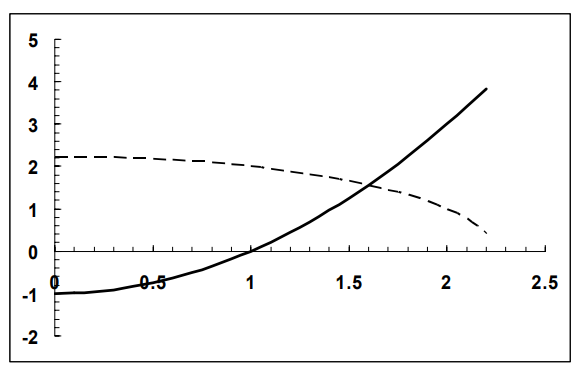
\includegraphics[width=0.5\linewidth]{fig_11_1}
		\label{fig:fig_11_1}
	\end{figure}
\bigbreak
Thus, a solution seems to lie at about $x=y=1.6$.
\bigbreak

\item The equations can be solved in a number of different ways. For example, the first equation can be solved for $x$ and the second solved for $y$. For this case, successive substitution does not work
\bigbreak

\underline{First iteration:}\\
$x=\sqrt{5-y^{2}}=\sqrt{5-(1.5)^{2}}=1.658312$
\\
$y=(1.658312)^{2}-1=1.75$
\bigbreak
\underline{Second iteration:}\\
$x=\sqrt{5-(1.75)^{2}}=1.391941$
\\
$y=(1.391941)^{2}-1=0.9375$
\bigbreak
\underline{Third iteration:}\\
$x=\sqrt{5-(0.9375)^{2}}=2.030048$
\\
$y=(2.030048)^{2}-1=3.12094$
\bigbreak
Thus, the solution is moving away from the solution that lies at approximately $x=y=1.6$.
\bigbreak
An alternative solution involves solving the second equation for $x$ and the first for $y$.\\ For this case, successive substitution does work
\bigbreak
\underline{First iteration:}\\
$x=\sqrt{y+1}=\sqrt{1.5+1}=1.581139$
\\
$y=\sqrt{5-x^{2}}=\sqrt{5-(1.581139)^{2}}=1.581139$
\bigbreak
\underline{Second iteration:}\\
$x=\sqrt{1.581139}=1.606592$
\\
$y=\sqrt{5-(1.606592)^{2}}=1.555269$
\bigbreak
\underline{Third iteration:}\\
$x=\sqrt{5-(1.555269)^{2}}=1.598521$ 
\\
$y=(1.598521)^{2}-1=1.563564$

\bigbreak
After several more iterations, the calculation converges on the solution of $x=1.600485$ and $y=1.561553 .$
\bigbreak
\item The equations to be solved are
\bigbreak$
\begin{aligned}
&f_{1}(x, y)=x^{2}-y-1 \\
&f_{2}(x, y)=5-y^{2}-x^{2}
\end{aligned}$
\bigbreak
The partial derivatives can be computed and evaluated at the initial guesses
\bigbreak
$\begin{array}{ll}
\dfrac{\partial f_{1,0}}{\partial x}=2 x &\quad\quad\quad\quad\quad \dfrac{\partial f_{1,0}}{\partial y}=-1 \\\\
\dfrac{\partial f_{2,0}}{\partial x}=-2 x &\quad\quad\quad\quad\quad \dfrac{\partial f_{2,0}}{\partial y}=-2 y
\end{array}$
\bigbreak
They can then be used to compute the determinant of the Jacobian for the first iteration is
\bigbreak
-1.4(-7)-(-1)(-3.6)=6.2
\bigbreak
The values of the functions can be evaluated at the initial guesses as
\bigbreak$
\begin{aligned}
&f_{1,0}=-1.2^{2}+1.2+0.5-1.2=-0.94 \\
&f_{2,0}=1.2^{2}-5(1.2)(1.2)-1.2=-6.96
\end{aligned}$
\bigbreak
These values can be substituted into Eq. (11.12) to give
\bigbreak
$\begin{aligned}
&x_{1}=1.2-\dfrac{-0.94(-3.6)-(-6.96)(-1)}{6.2}=1.26129 \\\\
&x_{2}=1.2-\dfrac{-6.96(-1.4)-(-0.94)(-3.6)}{6.2}=0.174194
\end{aligned}$
\bigbreak
The computation can be repeated until an acceptable accuracy is obtained.\\ The results are summarized as
\bigbreak
\begin{tabular}{crrrr}
\Xhline{1.5pt}
iteration & \multicolumn{1}{c}{$\xi$} & \multicolumn{1}{c}{$\psi$} & $\varepsilon_{\mathrm{a} 1}$ & $\varepsilon_{\mathrm{a} 2}$ \\
\hline
0 & $1.5$ & $1.5$ &  &  \\
1 & $1.604167$ & $1.5625$ & $6.494 \%$ & $4.000 \%$ \\
2 & $1.600489$ & $1.561553$ & $0.230 \%$ & $0.061 \%$ \\
3 & $1.600485$ & $1.561553$ & $0.000 \%$ & $0.000 \%$ \\
\Xhline{1.5pt}
\end{tabular}






\end{enumerate}
\end{document}


